\documentclass[11pt,border=5pt]{standalone}
\usepackage{fontspec}
\setmainfont{cmunrm.otf}[BoldFont=cmunbx.otf,ItalicFont=cmunti.otf,BoldItalicFont=cmunbi.otf]
\usepackage{amsmath}
\usepackage{unicode-math}
\setmathfont{NewCMMath-Regular.otf}
\usepackage{tikz}
\usetikzlibrary{arrows.meta,patterns,angles,quotes}
\begin{document}
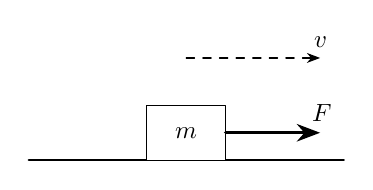
\begin{tikzpicture}[>=Stealth,font=\small,line cap=round,line join=round]
\draw[thick] (-2,0) -- (2,0);
\draw[fill=white] (-0.5,0.0) rectangle (0.5,0.7);
\node at (0,0.35) {$m$};
\draw[->,thin,dashed] (0,1.3) -- (1.7,1.3) node[above] {$v$};
\draw[->,very thick] (0.5,0.35) -- (1.7,0.35) node[above] {$F$};

\end{tikzpicture}
\end{document}
